In order to advect particles along with the flow field, one just needs to
add the \texttt{particles} postprocessor to the list of postprocessors and specify
a few parameters. We do so in the
\url{cookbooks/composition_passive_particles/composition_passive_particles.prm} input file, which is otherwise
just a minor variation of the \url{cookbooks/composition_passive/composition_passive.prm} case
discussed in the previous Section~\ref{sec:cookbooks-composition}. In
particular, the postprocess section now looks like this:

\index[prmindex]{Number of particles}
\index[prmindexfull]{Postprocess!Particles!Number of particles}

\lstinputlisting[language=prmfile]{particles.part.prm.out}

The 1000 particles we are asking here are initially uniformly distributed
throughout the domain and are, at the end of each time step, advected along with
the velocity field just computed. (There are a number of options to decide which
method to use for advecting particles, see
Section~\ref{parameters:Postprocess/Particles}.)

If you run this cookbook, information about all particles will be written into
the output directory selected in the input file (as discussed in
\index[prmindex]{Output directory}
\index[prmindexfull]{Output directory}
Section~\ref{sec:running-overview}). In the current case, in addition to the
files already discussed there, a directory listing at the end of a run will show
several particle related files:
\begin{lstlisting}[frame=single,language=ksh]
aspect> ls -l output/
total 932
-rw-rw-r-- 1 bangerth bangerth  11134 Dec 11 10:08 depth_average.gnuplot
-rw-rw-r-- 1 bangerth bangerth  11294 Dec 11 10:08 log.txt
-rw-rw-r-- 1 bangerth bangerth 326074 Dec 11 10:07 parameters.prm
-rw-rw-r-- 1 bangerth bangerth 577138 Dec 11 10:07 parameters.tex
drwxrwxr-x 2 bangerth bangerth   4096 Dec 11 18:40 particles
-rw-rw-r-- 1 bangerth bangerth    335 Dec 11 18:40 particles.pvd
-rw-rw-r-- 1 bangerth bangerth    168 Dec 11 18:40 particles.visit
drwxr-xr-x 2 bangerth bangerth   4096 Dec 11 10:08 solution
-rw-rw-r-- 1 bangerth bangerth    484 Dec 11 10:08 solution.pvd
-rw-rw-r-- 1 bangerth bangerth    451 Dec 11 10:08 solution.visit
-rw-rw-r-- 1 bangerth bangerth   8267 Dec 11 10:08 statistics
\end{lstlisting}
Here, the \texttt{particles.pvd} and \texttt{particles.visit} files contain
a list of all visualization files from all processors and time steps. These
files can be loaded in much the same way as the \texttt{solution.pvd} and
\texttt{solution.visit} files that were discussed in Section~\ref{sec:viz}. The
actual data files -- possibly a large number, but not of much immediate interest
to users -- are located in the \texttt{particles} subdirectory.

Coming back to the example at hand, we can visualize the particles that
were advected along by opening both the field-based output files and the ones
that correspond to particles (for example, \texttt{output/solution.visit} and
\texttt{output/particles.visit}) and using a pseudo-color plot
for the particles, selecting the ``id'' of particles to color each particle.
By going to, for example, the output from the 72nd visualization output, this
then results in a plot like the one shown in
Fig.~\ref{fig:composition_passive_particles}.

\begin{figure}
  \centering
  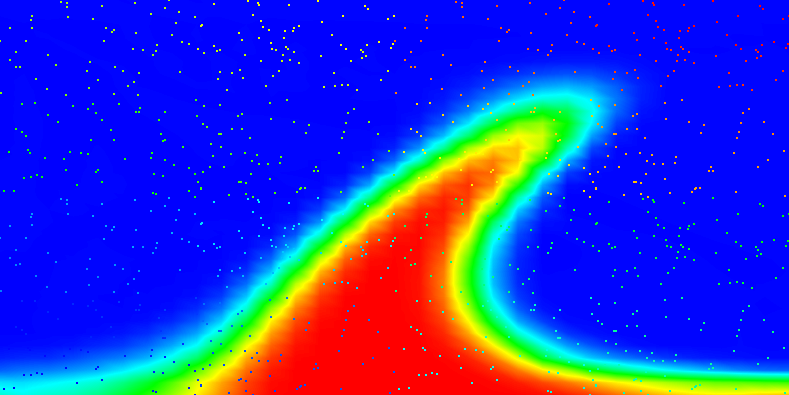
\includegraphics[width=0.5\textwidth]{solution-00072.png}
  \caption{\it Passively advected quantities visualized through both a
  \label{fig:composition_passive_particles}
  compositional field and a set of 1,000 particles, at $t=7.2$.}
\end{figure}

The particles shown here are not too impressive in still pictures since they are
colorized by their particle number, which does not carry any particular meaning
other than the fact that it enumerates the particles.%
\footnote{Particles are enumerated in a way so that first the first processor
in a parallel computations numbers all of the particles on its first cell, then
its second cell, and so on; then the second processor does the same with
particles in the order of the cells it owns; etc. Thus, the ``id'' shown in the
picture is not just a random number, but rather shows the order of cells and
how they belonged to the processors that participated in the computation at the
time when particles were created. After some time, particles may of course have
become well mixed. In any case, this ordering is of no real practical use.}
The particle ``id'' can, however, be useful when viewing an animation of time steps.
There, the different colors of particles allows the eye to follow the motion of
a single particle. This is especially true if, after some time, particles have
become well mixed by the flow field and adjacent particles no longer have
similar colors. In any case, viewing such animations makes it rather intuitive
to understand a flow field, but it can of course not be reproduced in a static medium such as this manual.

In any case, we will see in the next section how to attach more interesting
information to particles, and how to visualize these.

\paragraph{Using particle properties.}

The particles in the above example only fulfill the purpose of
visualizing the convection pattern. A more meaningful use for
particles is to attach ``properties'' to them. A property consists of
one or more numbers (or vectors or tensors) that may either be set at
the beginning of the model run and stay constant, or are updated
during the model runtime. These properties can then be used for many
applications, e.g., storing an initial property (like the position, or
initial composition), evaluating a property at a defined particle path (like the
pressure-temperature evolution of a certain piece of rock), or by integrating a
quantity along a particle path (like the integrated strain a certain domain has
experienced).  We illustrate these properties in the cookbook
\url{cookbooks/composition_passive_particles/composition_passive_particles_properties.prm}, in which we add the
following lines to the \texttt{Particles} subsection (we also increase the number
of particles compared to the previous section to make the visualizations below
more obvious):

\lstinputlisting[language=prmfile]{particle-properties.part.prm.out}

These commands make sure that every particle will carry four different
properties (\texttt{function}, \texttt{pT path}, \texttt{initial
  position} and \texttt{initial composition}), some of which may be
scalars and others can have multiple components. (A full list of
particle properties that can currently be selected can be found in
Section~\ref{parameters:Postprocess/Particles}, and new particle
properties can be added as plugins as described in
Section~\ref{sec:write-plugin}.) The properties selected above do the following:

\begin{itemize}
\item \texttt{initial position:} This particle property simply stores
  the initial coordinates of the particle and then never changes them. This
  can be useful to compare the final position of a particle with its
  initial position and therefore determine how far certain domains traveled
  during the model runtime. Alternatively, one may want to simply visualize
  the norm of this vector property (i.e., the norm of the initial position,
  which is of course equal to the distance from the origin at which a particle
  started): in mantle simulations in spherical coordinates, the radius is
  indicative of which part of the mantle a particle comes from, and can
  therefore be used to visualize where material gets transported over the course
  of a simulation.
\item \texttt{initial composition:} This property uses the same
  method to initialize particle properties as is used to initialize
  the corresponding compositional fields. Using this, it stores the
  compositional field initialization values at the location where the particle
  started, and again never changes them. This is useful in the same
  context as shown for the field-based example in
  Section~\ref{sec:cookbooks-composition} where we would like to
  figure where materials ends up. In this case, one would set the
  initial composition to an indicator function for certain parts of
  the domain, and then set the initial composition property for the
  particles to match this composition. Letting the particles advect
  and at a later time visualizing this particle property will then
  show where particles came from. In cases where compositional
  variables undergo changes, e.g., by describing phase changes or
  chemical reactions, the ``initial composition'' property can also be
  useful to compare the final composition of a particle with its
  initial composition and therefore determine which regions underwent
  reactions such as those described in Section~\ref{sec:cookbooks-composition},
  and where the material that underwent this reaction got transported
  to.
\item \texttt{function:} This particle property can be used to assign
  to each particle values that are described based on a function of
  space. It provides an alternative way to set initial values if you
  don't want to first set a compositional field's initial values based
  on a function, and then copy these values via the ``initial
  composition'' property to particles. In the example above, we use
  the same function as for the compositional initial composition of
  field number one in
  Section~\ref{sec:cookbooks-composition}. Therefore, this property
  should behave identical to the compositional field (except that the
  compositional field may have a reaction term that this particle
  property does not), although the two are of course advected using
  very different methods. This allows to compare the error in particle
  position to the numerical diffusion of the compositional field.
\item \texttt{pT path:} This property is interesting in that the
  particle property's values always exactly mirror the pressure and
  temperature at the particle's current location. This does not seem
  to be very useful since the information is already
  available. However, because each particle has a unique id, one can
  select a particular particle and output its properties
  (including pressure and temperature based on the \texttt{pT path}
  property) at all time steps. This allows for the creation of a pressure-temperature 
  curve of a certain piece of rock. This property is interesting in many lithosphere 
  and crustal scale models, because it is determining the metamorphic reactions that 
  happen during deformation processes (e.g., in a subduction zone).
\end{itemize}


\begin{figure}
  \centering
  \phantom{.}
  \hfill
  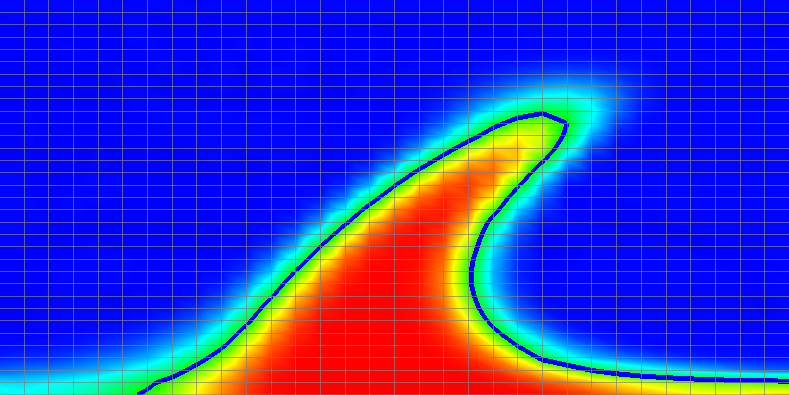
\includegraphics[width=0.45\textwidth]{composition-C1.png}
  \hfill
  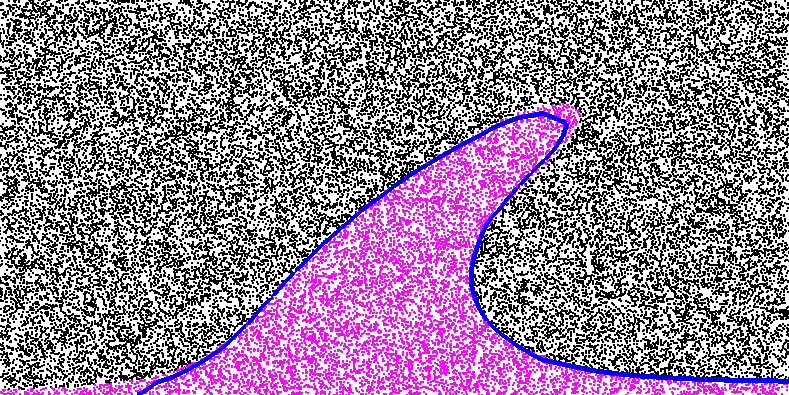
\includegraphics[width=0.45\textwidth]{particles-C1.png}
  \phantom{.}
  \\
  \phantom{.}
  \hfill
  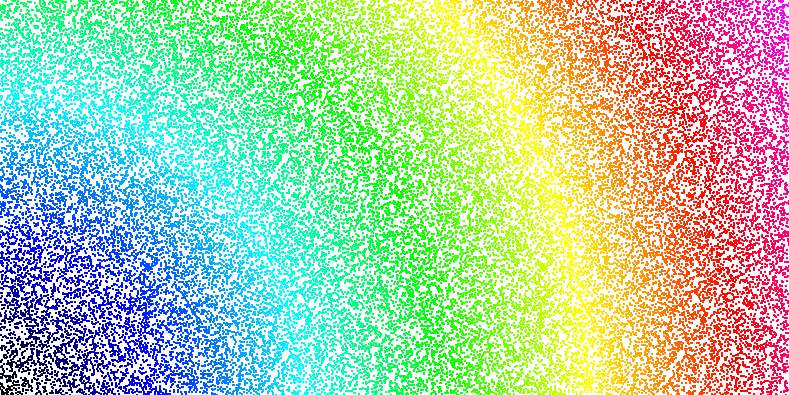
\includegraphics[width=0.45\textwidth]{initial-position-00000.png}
  \hfill
  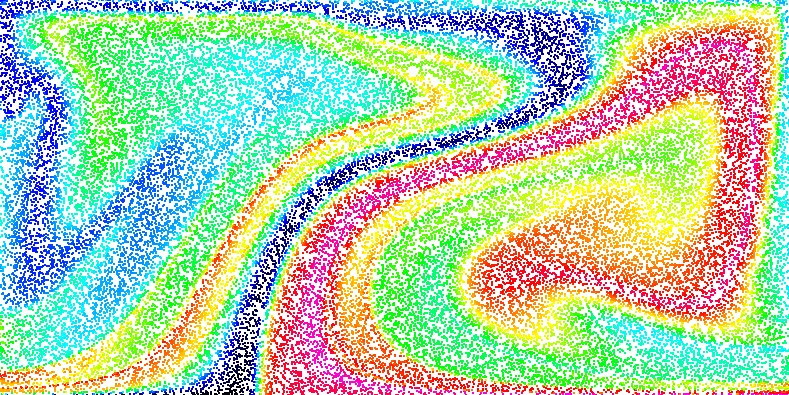
\includegraphics[width=0.45\textwidth]{initial-position-00199.png}
  \phantom{.}
  \caption{\it Passively advected particle properties visualized. Top row:
  Composition $C_1$ and particle property ``initial $C_1$''. The blue line in both
  figures is the 0.5-isocontour for the $C_1$ field. Bottom row: Norm of the
  ``initial position'' of particles at $t=0$ and $t=20$.}
  \label{fig:composition_passive_particles_properties}
\end{figure}

The results of all of these properties can of course be visualized.
Fig.~\ref{fig:composition_passive_particles_properties} shows some of the pictures
one can create with particles.
The top row shows both the composition field $C_1$ (along with the mesh on
which it is defined) and the corresponding ``initial $C_1$'' particle property,
at $t=7.2$. Because the compositional field does not undergo any reactions, it should of
course simply be the initial composition advected along with the flow field,
and therefore equal the values of the corresponding particle property. However,
field-based compositions suffer from diffusion. On the other hand, the amount
of diffusion can easily be decreased by mesh refinement.

The bottom of the figure shows the norm of the ``initial position'' property at
the initial time and at time $t=20$. These images therefore show how far from
the origin each of the particles shown was at the initial time.
